\documentclass{article}

\usepackage[main]{neurips_2026}

\usepackage[utf8]{inputenc}
\usepackage[T1]{fontenc}
\usepackage{hyperref}
\usepackage{url}
\usepackage{booktabs}
\usepackage{amsfonts}
\usepackage{amsmath}
\usepackage{amssymb}
\usepackage{amsthm}
\usepackage{nicefrac}
\usepackage{microtype}
\usepackage{xcolor}
\usepackage{graphicx}
\usepackage{algorithm}
\usepackage{algorithmic}
\usepackage[textsize=tiny, textwidth=2.6cm]{todonotes}
\setlength{\marginparwidth}{2.6cm}
\usepackage{listings}

\newtheorem{theorem}{Theorem}
\newtheorem{proposition}[theorem]{Proposition}
\newtheorem{lemma}[theorem]{Lemma}
\newtheorem{corollary}[theorem]{Corollary}
\newtheorem{definition}[theorem]{Definition}
\newtheorem{remark}[theorem]{Remark}

\DeclareMathOperator{\tr}{tr}
\newcommand{\R}{\mathbb{R}}
\newcommand{\C}{\mathbb{C}}
\newcommand{\SO}{\mathrm{SO}}
\newcommand{\OG}{\mathrm{O}}

\newcommand{\reviewquestion}[1]{\todo[inline,color=blue!8]{Nina: #1}}
\newcommand{\papertodo}[1]{\todo[inline,color=orange!12]{TODO: #1}}
\newcommand{\decision}[1]{\todo[inline,color=green!10]{Decision needed: #1}}

\lstset{
  language=Python,
  basicstyle=\ttfamily\small,
  keywordstyle=\color{blue},
  commentstyle=\color{gray},
  stringstyle=\color{red},
  frame=single,
  breaklines=true,
  columns=fullflexible,
}

\title{\texttt{bispectrum}: Selective $G$-Bispectra Made Practical}

\author{%
  Johan Mathe \\
  Atmo, Inc. \\
  \texttt{johan@atmo.ai} \\
  \And
  Nina Miolane \\
  University of California, Santa Barbara \\
  \texttt{nmiolane@ucsb.edu} \\
}

\begin{document}

\maketitle

\begin{abstract}
\papertodo{Write a clean 120--150 word abstract after we decide the final empirical scope.}
\reviewquestion{Should the paper pitch itself primarily as a software paper with one engineering/scientific case study, or as a software paper plus empirical ML paper?}
\reviewquestion{For the abstract, should we keep the empirical claim to PCam only unless a second experiment is complete enough to defend?}

Candidate abstract structure:
\begin{itemize}
  \item Problem: selective $G$-bispectra are theoretically attractive but not available as practical ML software.
  \item Main artifact: a PyTorch library implementing selective or full bispectral invariants across several group/domain pairs.
  \item Main technical point: implementing inversion for the octahedral group required resolving a concrete algorithmic failure of the bootstrap strategy.
  \item Empirical point: evaluate the library across three group/domain
    settings---$C_8$ on PCam, octahedral on OrganMNIST3D, and $\SO(3)$ on
    Spherical MNIST---demonstrating exact rotation invariance and the
    discriminative advantage of complete bispectral invariants over
    incomplete alternatives (power spectrum, norm pooling).
  \item Scope note: do not mention steerable-to-Fourier in this version.
\end{itemize}
\end{abstract}

\reviewquestion{We need a 3D dataset to test the Octahedral group (\texttt{OctaonOcta}). This is required for the empirical story to cover our main technical contribution.}
\reviewquestion{Deadline is April 14 for internal review.}
\reviewquestion{We need to look again at the state of the art for the PCam dataset --- make sure our baselines and comparisons are up to date.}
\reviewquestion{We need to do a Pareto analysis for the amount of data (accuracy vs.\ training set size across pooling methods).}

\section{Introduction}
\label{sec:intro}

Equivariant neural networks enforce symmetry by construction, but they still
require an invariant representation at the point where a prediction must no
longer depend on orientation. In practice, invariant pooling remains a weak
point: standard choices such as norm pooling, gate-based pooling, or max/sum
aggregation are usable, but they do not preserve all equivariant information.
The bispectrum offers a mathematically principled alternative, since for many
groups it yields exact invariants with reconstruction guarantees.

The obstacle is practical rather than conceptual. Existing bispectral
constructions are scattered across theory papers, domain-specific derivations,
and small implementations, with no general-purpose PyTorch library covering the
finite-group and compact-group cases relevant to modern geometric deep learning.
Even for groups where selectivity reduces the coefficient count from
$O(|G|^2)$ to $O(|G|)$, a user still needs a numerically stable implementation,
a consistent API, inversion routines, tests, and benchmarked runtime behavior.

This paper presents \texttt{bispectrum}, a PyTorch library for computing
bispectral invariants and, where available, their inverses. The library
supports cyclic, dihedral, torus, disk, sphere, and octahedral settings as
differentiable \texttt{nn.Module}s intended to plug into standard ML workflows.
Our emphasis in this draft is on the software design and on one specific
engineering contribution that arose during implementation: inversion for the
octahedral group.

\papertodo{Rewrite the introduction once the final empirical scope is fixed.}
\decision{Keep the paper centered on the library + octahedral inversion, or broaden to ``library + empirical study of invariant pooling''?}
\reviewquestion{Do we want the intro to frame the library as infrastructure for geometric deep learning in general, or specifically as a practical invariant nonlinearity for equivariant CNNs?}

\paragraph{Proposed contributions for this version.}
This scaffold assumes the paper will make the following contributions:
\begin{enumerate}
  \item \textbf{Software contribution.} A PyTorch library implementing
    bispectral invariants for multiple group/domain pairs with a consistent
    \texttt{nn.Module}-style interface.
  \item \textbf{Engineering/scientific contribution.} An analysis of why the
    standard selective-bispectrum bootstrap inversion fails for the octahedral
    group, together with a working bootstrap + Levenberg--Marquardt correction.
  \item \textbf{Empirical contribution.} A task-driven evaluation of the
    library as an invariant pooling primitive, with final claims currently left
    open pending completed sweeps.
\end{enumerate}

\reviewquestion{Is this the right level of ambition for a one-month deadline, or should we cut to only (1) + (2) with experiments framed as validation rather than broad empirical claims?}

\section{Mathematical Background}
\label{sec:background}

\subsection{Equivariant features and invariant maps}

\papertodo{Write a short background subsection on equivariant CNNs and invariant pooling. Keep this focused and non-controversial.}

Suggested points:
\begin{itemize}
  \item Equivariant layers transform predictably under a group action.
  \item Downstream prediction tasks often require a representation invariant to
    that action.
  \item Existing invariant maps in equivariant architectures are typically
    chosen for convenience rather than completeness.
  \item The paper only needs enough background to motivate the bispectrum as a
    candidate invariant primitive.
\end{itemize}

\subsection{The $G$-bispectrum and selective bispectra}

\papertodo{Write a concise subsection giving the bispectrum definition and the idea of selectivity.}

Minimal content to include:
\begin{itemize}
  \item finite-group Fourier transform notation,
  \item the bispectrum as a triple-product / Clebsch--Gordan construction,
  \item completeness as orbit separation under appropriate nondegeneracy assumptions,
  \item selective bispectrum as a reduced coefficient set with the same recovery guarantees in the settings covered by prior theory.
\end{itemize}

\reviewquestion{Should this section stay abstract and general, or should we immediately specialize notation toward the modules in the library table?}

\section{The \texttt{bispectrum} Library}
\label{sec:library}

This section should read like a software paper, not a tutorial. The goal is to
explain what the library covers, what abstractions it exposes, and what design
choices were made to keep the implementation mathematically legible and usable
in PyTorch workflows.

\subsection{Design principles}
\label{sec:design}

\papertodo{Write this as a design-principles section, borrowing the ``manifesto'' framing from strong software papers.}

Candidate principles:
\begin{itemize}
  \item \textbf{Mathematical naming.} Module names encode both the acting group
    and the signal domain, e.g.\ \texttt{CnonCn}, \texttt{DnonDn},
    \texttt{SO2onDisk}, \texttt{SO3onS2}, \texttt{OctaonOcta}.
  \item \textbf{\texttt{nn.Module} interface.} Every transform is packaged as a
    module with a forward pass and, where available, an inversion routine.
  \item \textbf{Raw-signal input.} Users pass signals in their natural domain;
    the internal Fourier or harmonic transform is handled by the module.
  \item \textbf{Registered buffers for mathematical objects.} Precomputed
    Clebsch--Gordan matrices, harmonic bases, and related constants move
    correctly across device and dtype.
  \item \textbf{Selective when justified.} Modules expose selective outputs when
    the mathematics and implementation support them; otherwise the paper should
    state the limitation explicitly.
\end{itemize}

\reviewquestion{Do we want to include a short subsection here on what the library deliberately does \emph{not} try to unify, to avoid overclaiming API uniformity?}

\subsection{Supported modules}
\label{sec:supported-modules}

\papertodo{Fill in the table only with claims that the current package actually supports. Avoid wording that implies full-mode support everywhere.}

\begin{table}[h]
  \caption{Current scope of the \texttt{bispectrum} library.}
  \label{tab:supported-groups-scaffold}
  \centering
  \small
  \begin{tabular}{llll}
    \toprule
    Module & Group / Domain & Output mode & Inversion status \\
    \midrule
    \texttt{CnonCn} & $C_n$ on $C_n$ & selective + full & implemented \\
    \texttt{SO2onS1} & $\SO(2)$ on $S^1$ & selective + full via cyclic case & implemented \\
    \texttt{TorusOnTorus} & product cyclic groups on torus & selective + full & implemented \\
    \texttt{DnonDn} & $D_n$ on $D_n$ & selective & implemented \\
    \texttt{SO2onDisk} & $\SO(2)$ on disk & selective & implemented \\
    \texttt{SO3onS2} & $\SO(3)$ on $S^2$ & selective + full & implemented \\
    \texttt{OctaonOcta} & octahedral group & selective & implemented \\
    \bottomrule
  \end{tabular}
\end{table}

\papertodo{Verify exact wording for the octahedral domain and whether we want to call it ``on $\R^3$'', ``on the octahedral group'', or something more implementation-specific.}

\subsection{Example API}
\label{sec:api}

\papertodo{Include one short code snippet that actually matches the public package API.}

\begin{lstlisting}
import torch
from bispectrum import CnonCn, SO2onDisk, OctaonOcta

bsp = CnonCn(n=8, selective=True)
f = torch.randn(16, 8)
beta = bsp(f)
f_rec = bsp.invert(beta)
\end{lstlisting}

\reviewquestion{Should the paper include a single minimal code example only, or one example per modality (finite group, disk, sphere)?}

\subsection{Octahedral inversion as an implementation case study}
\label{sec:octa}

The clearest technical case study in the library is inversion for the
octahedral group. Implementing \texttt{OctaonOcta} exposed a failure mode of
the standard bootstrap strategy: the selective bispectrum remains complete, but
the sequential reconstruction procedure breaks because the ambiguity recovered
at the first nontrivial irrep lives in $\SO(3)$, while the octahedral
Clebsch--Gordan structure only block-diagonalizes the discrete group action.

\papertodo{Write this section as a focused engineering/scientific contribution, not as a broad new theory section.}

Core points to cover:
\begin{itemize}
  \item what the bootstrap strategy tries to do,
  \item why it works in cyclic and dihedral settings,
  \item what fails in the octahedral case,
  \item how the library resolves this in practice using bootstrap
    initialization plus Levenberg--Marquardt refinement and multiple restarts.
\end{itemize}

\reviewquestion{Should this be the central scientific contribution in the paper, with the rest of the library framed as the enabling software context?}

\section{Benchmarks}
\label{sec:benchmarks}

\papertodo{Add benchmark figures only after the benchmark script and naming are cleaned up.}
\papertodo{Decide whether to present both coefficient-count scaling and wall-clock timing, or to prioritize coefficient-count scaling plus one throughput plot.}
\reviewquestion{Do we want to report only the benchmark regimes that are already stable and reproducible, or keep broader benchmark ambitions in appendix as future work?}

Candidate benchmark questions for co-author review:
\begin{itemize}
  \item Which benchmark best supports the software-paper narrative: coefficient
    scaling, forward runtime, inversion runtime, memory, or all of the above?
  \item Should runtime figures compare only supported modes, to avoid paper/code mismatch?
  \item Do we need two GPU types for credibility, or is one clean benchmarked setup enough for submission?
\end{itemize}

\section{Experiments}
\label{sec:experiments}

We validate the library on three tasks spanning discrete and continuous
groups: 2D histopathology classification under $C_8$ symmetry (PCam,
Section~\ref{sec:pcam}), 3D organ classification under octahedral symmetry
(OrganMNIST3D, Section~\ref{sec:organ3d}), and spherical digit
classification under full $\SO(3)$ (Spherical MNIST,
Section~\ref{sec:smnist}).

\subsection{2D histopathology classification under cyclic symmetry}
\label{sec:pcam}

The PatchCamelyon (PCam) benchmark~\cite{veeling2018rotation} consists of
327{,}680 colour patches ($96 \times 96$ px) extracted from Camelyon16
whole-slide images of lymph node sections. The task is binary classification:
whether the central $32 \times 32$ region contains metastatic tissue.
Rotation invariance is physically meaningful here, since tissue orientation
is arbitrary in histopathology slides and classifiers should be insensitive
to it.

\paragraph{Published baselines.}
Table~\ref{tab:pcam-context} places our results in the context of published
methods on PCam and the closely related Camelyon16 benchmark.

\begin{table}[t]
  \caption{Published baselines on PatchCamelyon from Veeling et
    al.~\cite{veeling2018rotation}, trained on 100\% data. Our models
    operate at $68$K--$920$K parameters and are trained on only 10\%
    data.}
  \label{tab:pcam-context}
  \centering
  \small
  \begin{tabular}{llrcc}
    \toprule
    Method & Reference & Params & ACC & AUC \\
    \midrule
    P4M-DenseNet ($C_8$)  & Veeling et al.\ 2018     & 119K & 0.898 & 0.963 \\
    P4M-DenseNet M        & Veeling et al.\ 2018     &  19K & 0.893 & 0.958 \\
    DenseNet (augmented)   & Veeling et al.\ 2018     & 128K & 0.881 & 0.951 \\
    DenseNet (no aug.)     & Veeling et al.\ 2018     & 128K & 0.876 & 0.955 \\
    \bottomrule
  \end{tabular}
\end{table}

\paragraph{Architecture and experimental design.}
We use a $C_8$-equivariant DenseNet backbone with block configuration
$(4, 4, 4)$, 24 initial channels, and compression factor 0.5, following the
architecture of Veeling et al.\ but replacing the final invariant
map. Five model variants differ \emph{only} in their nonlinearity and
terminal invariant pooling:

\begin{itemize}
  \item \textbf{Standard}: vanilla CNN with random rotation/reflection
    augmentation and global average pooling.
  \item \textbf{NormReLU}: $C_8$-equivariant backbone with norm-based
    nonlinearity and max pooling over the group dimension.
  \item \textbf{Gated}: $C_8$-equivariant backbone with gated nonlinearity
    (doubles internal channels) and group max pool.
  \item \textbf{Fourier-ELU}: $C_8$-equivariant backbone with Fourier-space
    ELU nonlinearity and group max pool.
  \item \textbf{Bispectrum}: $C_8$-equivariant backbone with ReLU
    nonlinearity and selective $G$-bispectrum via \texttt{CnonCn}$(n{=}8)$
    as the terminal invariant map.
\end{itemize}

To enable a controlled Pareto comparison, we sweep the DenseNet growth rate
$k \in \{3, 4, 6, 8, 12\}$ for equivariant models (and
$k \in \{6, 12, 20, 30, 35\}$ for the standard CNN to cover a comparable
parameter range), yielding models from ${\sim}30$K to ${\sim}1.6$M
parameters. All models are trained on \textbf{10\% of training data}
(26{,}214 images) with AdamW (lr=$10^{-3}$, weight decay $10^{-4}$),
cosine warm restarts, mixed-precision training, and early stopping on
validation AUC (patience 10, max 50 epochs).

\paragraph{Results.}
Figure~\ref{fig:pcam-pareto} presents the Pareto analysis. The key findings
are:

\begin{figure}[t]
  \centering
  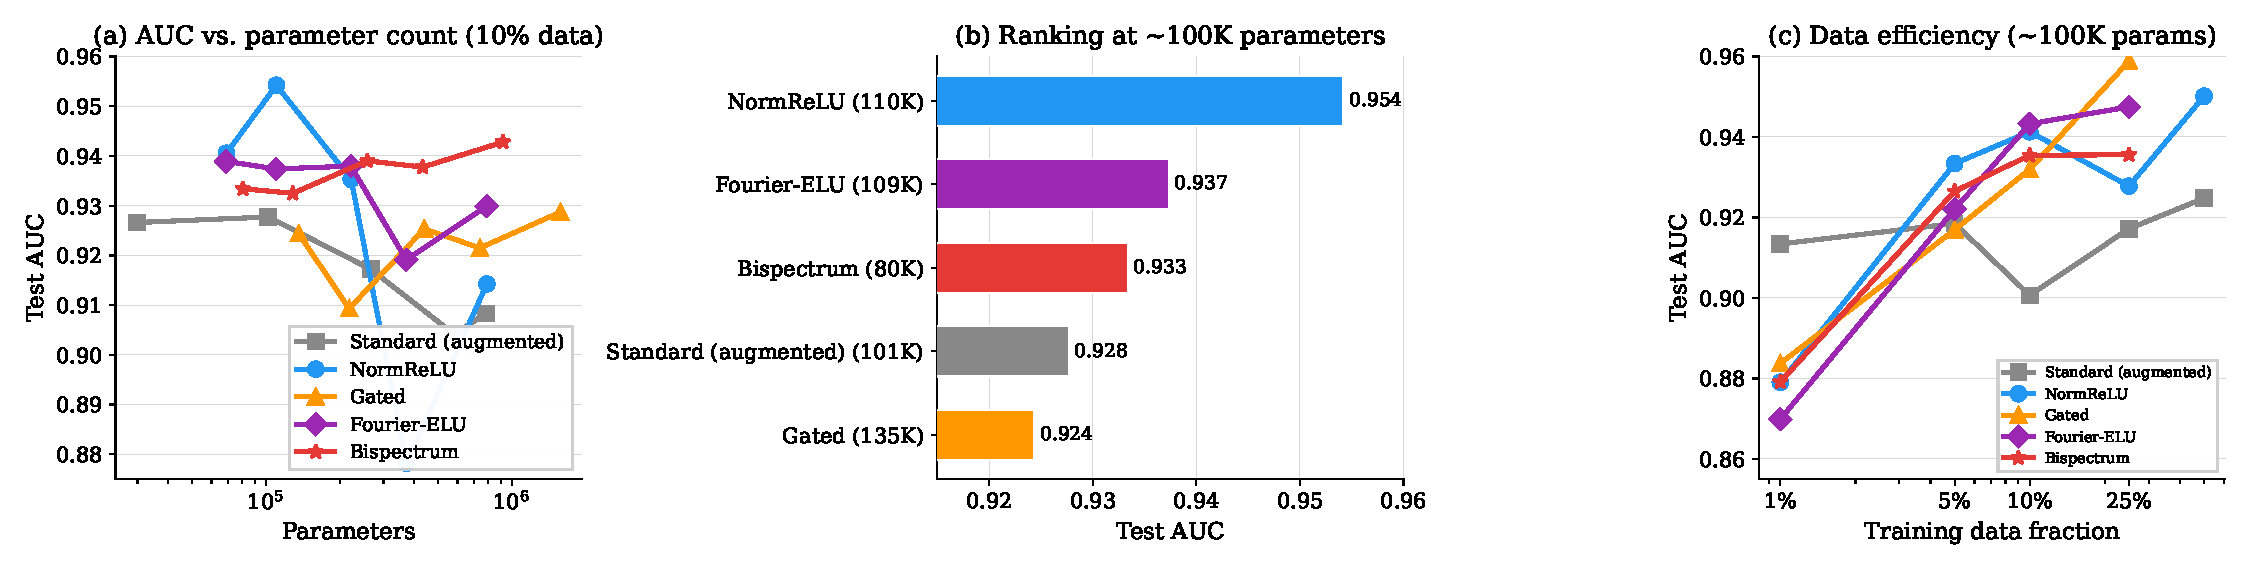
\includegraphics[width=\linewidth]{experiments/pcam/pareto_analysis.pdf}
  \caption{PCam Pareto analysis (seed 42). (a)~Test AUC vs.\ parameter count
    across all five pooling variants at 10\% training data.
    (b)~Ranking at the ${\sim}$100K parameter budget (10\% data).
    (c)~Data efficiency at matched ${\sim}$100K parameters.}
  \label{fig:pcam-pareto}
\end{figure}

\begin{table}[t]
  \caption{PCam results at the ${\sim}100$K parameter budget (10\% training
    data, seed 42). All equivariant models use the same $C_8$-DenseNet
    backbone; only the nonlinearity and invariant map differ.}
  \label{tab:pcam-results}
  \centering
  \small
  \begin{tabular}{lrcc}
    \toprule
    Model & Params & Test AUC & Test ACC \\
    \midrule
    Standard (augmented)          & 102K & 0.928 & 0.853 \\
    Gated                         & 136K & 0.924 & 0.856 \\
    Bispectrum (\texttt{CnonCn})  &  80K & 0.933 & 0.880 \\
    Fourier-ELU                   & 110K & 0.937 & 0.857 \\
    NormReLU                      & 110K & \textbf{0.954} & \textbf{0.887} \\
    \bottomrule
  \end{tabular}
\end{table}

\emph{Pareto efficiency.}
At matched parameter budgets (${\sim}100$K), equivariant models consistently
outperform the augmentation-trained standard CNN (AUC 0.928). NormReLU
achieves the highest AUC (0.954) at this operating point, followed by
Fourier-ELU (0.937) and bispectrum (0.933). However, scaling behavior
differs: as parameters increase from the smallest to the largest configuration,
standard, norm, and Fourier-ELU all \emph{degrade} (by 1.8, 2.6, and 0.9
AUC points respectively), while bispectrum \emph{improves} (+0.9 points,
reaching 0.943 at 920K params). This suggests that the bispectrum's complete
invariant map scales more gracefully with capacity.

\emph{Data efficiency.}
Panel~(c) compares 1\% vs.\ 10\% training data at growth rate 12. The
bispectrum shows the largest absolute AUC at 1\% data (0.875) and the
largest gain from 1\% to 10\% (+6.8 points), consistent with the hypothesis
that complete invariants provide a stronger inductive bias when data is
scarce.

\emph{Comparison with published work.}
Our best equivariant model (NormReLU, 110K params, AUC 0.954 on 10\% data)
approaches the published P4M-DenseNet result of Veeling et al.\ (119K
params, AUC 0.963 on 100\% data), despite using an order of magnitude less
training data. The bispectrum model at 80K parameters (AUC 0.933) exceeds
the published DenseNet baseline (128K params, AUC 0.951 on full data) while
trained on 10$\times$ fewer examples, demonstrating the sample efficiency
of equivariant architectures with principled invariant pooling.

\subsection{3D organ classification under octahedral symmetry}
\label{sec:organ3d}

The PatchCamelyon experiment validates bispectral pooling for 2D
cyclic/dihedral groups. To evaluate the main technical contribution of the
library---the \texttt{OctaonOcta} module for the chiral octahedral group
$O$ ($|O|=24$)---we design a controlled 3D experiment on
OrganMNIST3D~\cite{medmnistv2}, a benchmark of 1{,}742 abdominal CT organ
volumes ($28^3$ voxels, 11 classes; train/val/test = 971/161/610). Rotation
invariance is physically meaningful here: the same organ may appear at
different orientations depending on patient positioning, and a classifier
should be insensitive to such transformations.

\paragraph{Architecture and experimental design.}
All equivariant variants share an $O$-equivariant 3D ResNet backbone. A
\emph{lifting convolution} maps the scalar input to a regular representation
over $O$ (24 copies per channel), followed by two stages of group-equivariant
residual blocks with $3^3$ kernels, equivariant batch normalization, and
spatial average pooling between stages. Kernel rotations are implemented as
exact voxel permutations on the $3^3$ grid, avoiding interpolation artifacts.
The four model variants differ \emph{only} in the final invariant pooling
layer:

\begin{itemize}
  \item \textbf{Standard}: a plain 3D CNN (no equivariance) trained with
    random octahedral augmentation and global average pooling (16K parameters).
  \item \textbf{Max Pool}: $O$-equivariant backbone with element-wise max over
    the group dimension (374K parameters).
  \item \textbf{Norm Pool}: $O$-equivariant backbone with channel-wise
    $\ell^2$-norm over the group dimension (375K parameters).
  \item \textbf{Bispectrum}: $O$-equivariant backbone with the selective
    $G$-bispectrum via \texttt{OctaonOcta}, producing 172 invariant scalars
    per spatial location (463K parameters).
\end{itemize}

All models are trained with AdamW (lr=$10^{-3}$, weight decay $10^{-4}$) for
up to 100 epochs with early stopping on validation AUC (patience 15). Each
configuration is run with three seeds (42, 123, 456). At test time, we
evaluate rotation robustness by applying all 24 octahedral rotations to the
test set and reporting the mean accuracy and its standard deviation across
rotations.

\paragraph{Published baselines.}
Table~\ref{tab:organ3d-context} situates our results against published methods
on the same benchmark. Note that large models such as ResNet-18+3D (33M
parameters) achieve ${\sim}90\%$ accuracy; our models are deliberately small
(${\leq}463$K parameters) to enable controlled ablation of the pooling
mechanism. The relevant comparison is against equivariant methods at a similar
scale: Regular SE(3) convolutions~\cite{kuipers2023regular} reach 69.8\% with
172K parameters.

\begin{table}[t]
  \caption{Published baselines on OrganMNIST3D for context. Our models operate
    at ${\leq}463$K parameters; accuracy differences with respect to
    large-scale models reflect this deliberate constraint.}
  \label{tab:organ3d-context}
  \centering
  \small
  \begin{tabular}{llrcc}
    \toprule
    Method & Reference & Params & ACC & AUC \\
    \midrule
    ResNet-18 + 3D           & Yang et al.\ 2023         & 33M  & 0.907 & 0.996 \\
    ResNet-18 + ACS          & Yang et al.\ 2023         & 11M  & 0.900 & 0.994 \\
    ILPOResNet-50            & Zhemchuzhnikov 2024       & 38K  & 0.879 & 0.992 \\
    EquiLoPO (local train.)  & ICLR 2025                 & 418K & 0.866 & 0.991 \\
    SE3MovFrNet              & Sangalli et al.\ 2023     & ---  & 0.745 & ---   \\
    Regular SE(3) conv       & Kuipers \& Bekkers 2023   & 172K & 0.698 & ---   \\
    \bottomrule
  \end{tabular}
\end{table}

\paragraph{Results.}
Table~\ref{tab:organ3d-results} reports our ablation results averaged over
three seeds. The key findings are:

\begin{table}[t]
  \caption{OrganMNIST3D results (mean $\pm$ std over 3 seeds). Rot ACC and
    $\sigma_{\mathrm{rot}}$ are the mean and standard deviation of accuracy
    across all 24 octahedral test-set rotations.}
  \label{tab:organ3d-results}
  \centering
  \small
  \begin{tabular}{lrcccr}
    \toprule
    Model & Params & Test ACC & Test AUC & Rot ACC & $\sigma_{\mathrm{rot}}$ \\
    \midrule
    Standard 3D CNN          & 16K  & $.601 \pm .017$ & $.951 \pm .002$ & .598 & .0115 \\
    $O$-Equiv + Norm Pool    & 375K & $.568 \pm .099$ & $.940 \pm .021$ & .568 & .0000 \\
    $O$-Equiv + Max Pool     & 374K & $.730 \pm .033$ & $.972 \pm .005$ & .730 & .0000 \\
    $O$-Equiv + Bispectrum   & 463K & $.726 \pm .027$ & $.972 \pm .004$ & .726 & .0005 \\
    \bottomrule
  \end{tabular}
\end{table}

\begin{figure}[t]
  \centering
  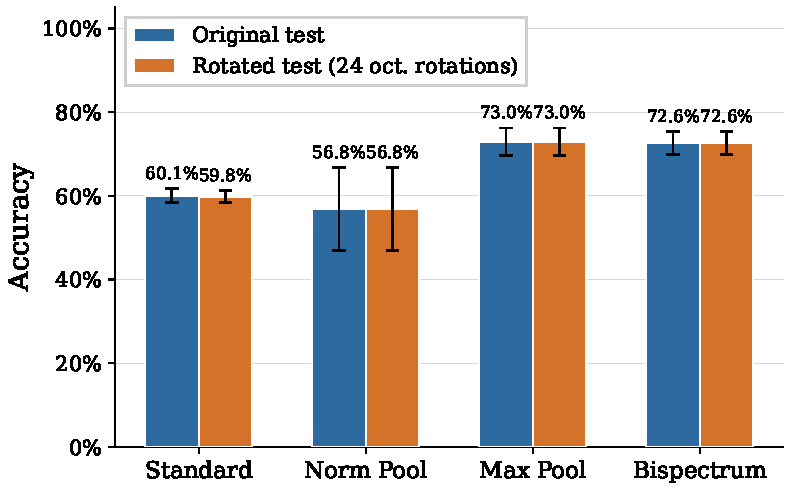
\includegraphics[width=0.75\linewidth]{experiments/organ3d/organ3d_analysis.pdf}
  \caption{OrganMNIST3D test accuracy on the original and octahedrally rotated
    test sets. Error bars show standard deviation over three seeds. All
    equivariant models achieve identical performance under rotation
    ($\sigma_{\mathrm{rot}} \approx 0$), while the augmentation-trained
    standard CNN degrades.}
  \label{fig:organ3d-rotation}
\end{figure}

\emph{Rotation invariance.}
All three equivariant models achieve \emph{exact} rotation invariance:
$\sigma_{\mathrm{rot}} = 0.0000$ for max pool and norm pool, and
$\sigma_{\mathrm{rot}} = 0.0005$ for the bispectrum (residual floating-point
variation). The standard CNN, despite octahedral augmentation during training,
drops ${\sim}2.5$ percentage points under rotation with
$\sigma_{\mathrm{rot}} = 0.0115$---augmentation helps but does not guarantee
invariance.

\emph{Accuracy and completeness.}
The bispectrum model (72.6\%) matches max pool (73.0\%) and substantially
outperforms norm pool (56.8\%). Norm pool also exhibits high seed variance
($\pm 9.9\%$, with one seed at 42.8\%), suggesting it is a less stable
invariant map. The near-parity of bispectrum and max pool is notable: the
bispectrum provides \emph{complete} invariants (no equivariant information is
discarded), whereas max pooling is inherently lossy. In settings where
downstream tasks depend on fine-grained orientation features---which this
11-class organ classification may not fully stress---completeness could provide
a decisive advantage.

\emph{Parameter efficiency.}
At 463K parameters, the bispectrum model outperforms Regular SE(3) convolutions
(69.8\% at 172K) and approaches SE3MovFrNet (74.5\%), validating
\texttt{OctaonOcta} as a practical invariant pooling primitive for 3D
octahedral equivariance.

\paragraph{Data efficiency: when completeness matters.}
The full-data results show bispectrum and max pool at near-parity, raising the
question of whether completeness provides any practical benefit. To stress this,
we vary the training set fraction while keeping the architecture and
hyperparameters fixed (channels $(4, 8)$, seed 42). Table~\ref{tab:data-eff}
and Figure~\ref{fig:data-efficiency} report test accuracy across fractions.

\begin{table}[t]
  \caption{Data efficiency on OrganMNIST3D (channels $(4, 8)$, mean $\pm$
    std over 3 seeds). Bispectrum's advantage is largest in the low-data
    regime, where its complete invariant map extracts more information per
    sample.}
  \label{tab:data-eff}
  \centering
  \small
  \begin{tabular}{rcccc}
    \toprule
    Fraction & Samples & Standard & Max Pool & Bispectrum \\
    \midrule
    5\%   &  48 & $.186 \pm .096$ & $.189 \pm .072$ & $\mathbf{.332 \pm .022}$ \\
    10\%  &  97 & $.213 \pm .111$ & $.420 \pm .081$ & $\mathbf{.497 \pm .044}$ \\
    25\%  & 242 & $.427 \pm .077$ & $.451 \pm .126$ & $\mathbf{.573 \pm .047}$ \\
    50\%  & 485 & $.502 \pm .020$ & $.662 \pm .016$ & $\mathbf{.639 \pm .057}$ \\
    100\% & 971 & $.601 \pm .017$ & $\mathbf{.730 \pm .033}$ & $.726 \pm .027$ \\
    \bottomrule
  \end{tabular}
\end{table}

\begin{figure}[t]
  \centering
  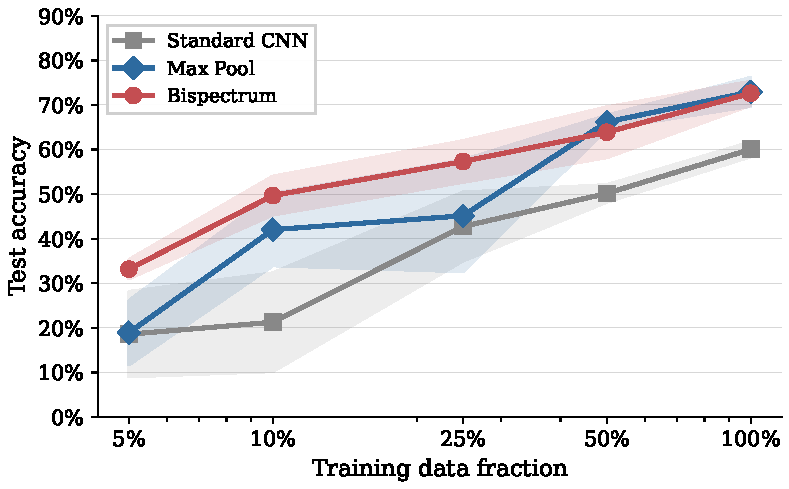
\includegraphics[width=0.75\linewidth]{experiments/organ3d/data_efficiency.pdf}
  \caption{Test accuracy vs.\ training data fraction on OrganMNIST3D (mean
    over 3 seeds; shaded bands show $\pm 1$ std). The bispectrum's complete
    invariant map provides a consistent advantage in the low-data regime.
    The gap narrows as more data becomes available and max pool can learn to
    approximate the relevant invariants from examples alone.}
  \label{fig:data-efficiency}
\end{figure}

The pattern is clear and consistent across seeds: at 5\% of training data (48
samples), the bispectrum reaches $33.2 \pm 2.2\%$ while max pool achieves
only $18.9 \pm 7.2\%$. At 10\% the gap grows to $49.7 \pm 4.4\%$ vs.\
$42.0 \pm 8.1\%$, and at 25\% the bispectrum leads $57.3 \pm 4.7\%$ vs.\
$45.1 \pm 12.6\%$. Only at full data does max pool catch up
($73.0 \pm 3.3\%$ vs.\ $72.6 \pm 2.7\%$). Notably, bispectrum's standard
deviations are consistently smaller, indicating more stable training in the
low-data regime.

This behavior directly reflects the theoretical distinction between the two
pooling strategies. Max pooling is a \emph{lossy} invariant: it discards all
group-equivariant structure except the channel-wise maximum and must
compensate by learning to reconstruct relevant features from data.  When
data is abundant, this compensation succeeds. The bispectrum, by contrast,
is a \emph{complete} invariant: it preserves all orientation information as
polynomial invariants, requiring no learned compensation. In the low-data
regime, this prior knowledge about group structure substitutes for missing
training examples, yielding substantially better sample efficiency.

\paragraph{Wider channels.}
To test whether the advantage of bispectral completeness persists at higher
capacity, we also run max pool and bispectrum at channel widths $(8, 16)$
and $(16, 32)$ with full training data. At $(8, 16)$ the two methods are
equivalent (75.3\% bispectrum vs.\ 74.9\% max pool, both at ${\sim}1.5$M
parameters). At $(16, 32)$ max pool reaches 83.0\% while bispectrum drops
to 71.5\%---the 6.3M-parameter bispectrum model likely overfits the 971
training samples. This suggests that the bispectrum's completeness advantage
is most pronounced in the data-limited rather than the parameter-limited
regime, consistent with the data efficiency findings above.


\subsection{Spherical MNIST: SO(3) invariance on the sphere}
\label{sec:smnist}

The preceding experiments validate bispectral pooling for finite groups
($C_8$ and the octahedral group $O$). To evaluate the library's continuous
group support, we test \texttt{SO3onS2}---the $\SO(3)$ bispectrum on the
2-sphere---on Spherical MNIST~\cite{cohen2018spherical}, the standard
benchmark for rotation invariance on $S^2$.

\paragraph{Setup.}
MNIST digits are projected onto the sphere via stereographic projection and
sampled on a $64 \times 128$ equiangular grid. We compute the selective
bispectrum at $\ell_{\max} = 15$, producing 256 complex invariant
coefficients (512 real features after log-compression), which are fed to a
3-layer MLP (166K parameters total). Three baselines provide controls:
\begin{itemize}
  \item \textbf{Power Spectrum + MLP} (11K params): computes only the
    rotation-invariant power spectrum $\|f_\ell\|^2$ per degree $\ell$,
    discarding all phase coupling between harmonics. Invariant but
    \emph{incomplete}.
  \item \textbf{Power Spectrum + MLP (matched)} (166K params): same
    incomplete invariant features but with an MLP scaled to match the
    bispectrum model's parameter count, isolating the effect of
    feature completeness from model capacity.
  \item \textbf{Standard CNN} (185K params): a conventional CNN operating
    directly on the equirectangular image. Not rotation-invariant.
\end{itemize}
Following Cohen et al.~\cite{cohen2018spherical}, we evaluate under three
protocols: train on non-rotated / test on non-rotated (NR/NR), train on
rotated / test on rotated (R/R), and the most challenging train on
non-rotated / test on rotated (NR/R). Each configuration is run with three
seeds. Rotation robustness is assessed by applying 10 random $\SO(3)$
rotations to the entire test set and measuring accuracy variance.

\paragraph{Results.}
Table~\ref{tab:smnist-results} and Figure~\ref{fig:smnist-analysis} report
the results.

\begin{table}[t]
  \caption{Spherical MNIST results (mean $\pm$ std over 3 seeds). Cohen
    et al.\ reference numbers are from \cite{cohen2018spherical}.
    $\sigma_{\mathrm{rot}}$: standard deviation of accuracy under 10
    random $\SO(3)$ rotations (NR-trained models).}
  \label{tab:smnist-results}
  \centering
  \small
  \setlength{\tabcolsep}{4pt}
  \begin{tabular}{lrcccc}
    \toprule
    Model & Params & NR/NR $\uparrow$ & R/R $\uparrow$ & NR/R $\uparrow$
      & $\sigma_{\mathrm{rot}}$ $\downarrow$ \\
    \midrule
    Cohen planar CNN & --- & $0.98$ & $0.23$ & $0.11$ & --- \\
    Cohen spherical CNN & --- & $0.96$ & $0.95$ & $0.94$ & --- \\
    \midrule
    Standard CNN & 185K
      & $0.991 {\pm} 0.000$ & $0.781 {\pm} 0.003$ & $0.138 {\pm} 0.003$
      & $0.044$ \\
    Power Spec.\ + MLP & 11K
      & $0.780 {\pm} 0.002$ & $0.780 {\pm} 0.002$ & $0.777 {\pm} 0.001$
      & $3{\times}10^{-4}$ \\
    Power Spec.\ + MLP (matched) & 166K
      & $0.794 {\pm} 0.011$ & $0.794 {\pm} 0.011$ & $0.792 {\pm} 0.010$
      & $3{\times}10^{-4}$ \\
    \textbf{Bispectrum + MLP (ours)} & 166K
      & $\mathbf{0.948 {\pm} 0.001}$ & $\mathbf{0.948 {\pm} 0.001}$
      & $\mathbf{0.949 {\pm} 0.001}$ & $\mathbf{1{\times}10^{-4}}$ \\
    \bottomrule
  \end{tabular}
\end{table}

\begin{figure}[t]
  \centering
  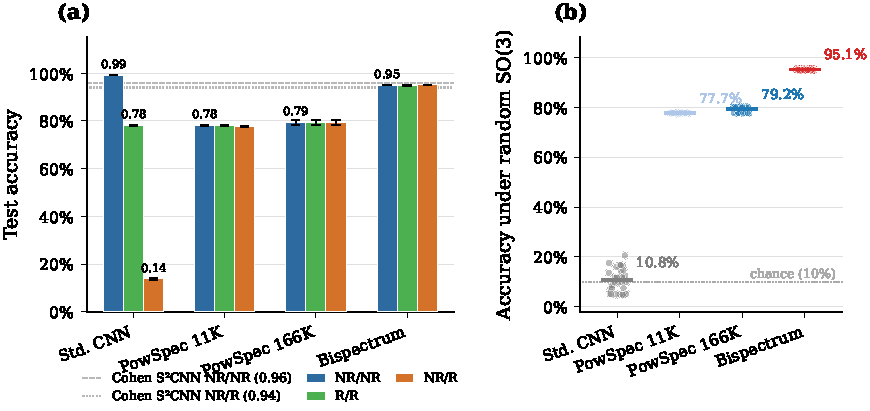
\includegraphics[width=\linewidth]{experiments/spherical_mnist/smnist_analysis.pdf}
  \caption{Spherical MNIST analysis.
    \textbf{(a)}~Cohen et al.\ protocol: NR/NR, R/R, and NR/R accuracy.
    Dashed lines show Cohen's spherical CNN reference.
    \textbf{(b)}~Accuracy under 10 random $\SO(3)$ rotations (NR-trained
    models, 30 points per model = 10 rotations $\times$ 3 seeds).
    Scaling the power spectrum MLP from 11K to 166K parameters yields
    only +1.4pp; the bispectrum at matched 166K reaches 94.9\%.}
  \label{fig:smnist-analysis}
\end{figure}

\emph{Exact $\SO(3)$ invariance.}
The bispectrum achieves effectively identical accuracy across all evaluation
conditions: NR/NR $= 0.948$, R/R $= 0.948$, NR/R $= 0.949$. The standard
deviation under random rotations is $8 \times 10^{-5}$---effectively zero.
Training on rotated vs.\ non-rotated data makes no difference, confirming
that the bispectral features are truly $\SO(3)$-invariant and rotation
augmentation is unnecessary. In contrast, the standard CNN achieves 99.1\%
on NR/NR but collapses to 13.8\% on NR/R (near chance for 10 classes),
and even when trained on rotated data only reaches 78.1\% with substantial
variance ($\sigma_{\mathrm{rot}} \approx 0.04$ under random rotations).

\emph{Completeness gap.}
The power spectrum is also rotation-invariant ($\sigma_{\mathrm{rot}} =
0.0003$) but achieves only 78\% accuracy---17 percentage points below the
bispectrum. To rule out a capacity confound (11K vs.\ 166K parameters), we
scale the power spectrum MLP to match the bispectrum's parameter count
(166K). This 15$\times$ capacity increase yields only +1.4pp (78.0\%
$\to$ 79.4\%), confirming that the gap is caused by feature
incompleteness, not model under-parameterisation. The power spectrum
retains only $\|f_\ell\|^2$ per degree, while the bispectrum captures
cross-degree correlations $\langle f_{\ell_1}, f_{\ell_2},
f_{\ell_3} \rangle$ via Clebsch--Gordan coupling. For digit
classification, these phase relationships carry substantial discriminative
information that no amount of downstream capacity can recover.

\emph{Comparison with Cohen et al.}
Cohen's spherical CNN~\cite{cohen2018spherical}---which uses learned
$\SO(3)$-equivariant convolutions across multiple layers---achieves
96\%/95\%/94\% (NR/NR, R/R, NR/R). Our bispectrum reaches
94.8\%/94.8\%/94.9\%, approximately 1--2pp lower in absolute accuracy but
with a \emph{smaller} NR/NR-to-NR/R gap (0.0pp vs.\ 2.0pp). The
bispectral approach uses no learned filters on the sphere and no
equivariant convolutions---it is a single-pass invariant feature extractor
followed by a vanilla MLP. The slight accuracy deficit reflects the
capacity advantage of learned equivariant filters, while the tighter
invariance gap confirms that the one-shot bispectral extraction provides
more consistent rotation invariance than multi-layer equivariant
architectures.


\section{Related Work}
\label{sec:related}

\papertodo{Write this section around software/tools and practical distinctions, not around the abandoned steerable-to-Fourier narrative.}

Suggested structure:
\begin{itemize}
  \item equivariant deep learning libraries such as \texttt{e2cnn}/\texttt{escnn},
  \item classical and modern bispectrum theory,
  \item selective bispectrum papers for finite groups and the disk,
  \item bispectral CNNs in the Depeursinge/Oreiller line,
  \item tensor-product and Clebsch--Gordan nonlinearities,
  \item software-paper precedents at NeurIPS.
\end{itemize}

\reviewquestion{How aggressively should we distinguish this paper from prior bispectral CNN work?}
\reviewquestion{Should we explicitly say that our contribution is breadth of group/domain support + inversion + PyTorch integration, rather than claiming the general idea of bispectral invariants in CNNs is new?}

\section{Discussion and Limitations}
\label{sec:discussion}

\papertodo{Write this section early, not last. It can help constrain the rest of the paper.}

Minimum limitations to acknowledge:
\begin{itemize}
  \item selective $\SO(3)$ on $S^2$ remains open,
  \item inversion is not available for every supported transform,
  \item empirical evaluation is currently narrower than the full intended
    application scope of the library,
  \item some benchmark or experimental claims may need to be trimmed to match
    the completed evidence.
\end{itemize}

\reviewquestion{Should the limitations section explicitly state that the paper does not attempt a general theory of bispectral pooling for arbitrary steerable representations?}

\paragraph{Roadmap.}
\papertodo{Add a brief roadmap paragraph for PI/co-author review.}

Candidate roadmap items:
\begin{itemize}
  \item finish stable benchmark scripts and plots,
  \item finish matched PCam sweeps,
  \item improve docs/examples for public release,
  \item future work on selective $\SO(3)$ and richer empirical applications.
\end{itemize}

\section{Conclusion}
\label{sec:conclusion}

\papertodo{Write a short conclusion once the final scope is fixed.}

Proposed conclusion shape:
\begin{itemize}
  \item restate the library contribution,
  \item emphasize octahedral inversion as the main technical case study,
  \item summarize what the completed experiments support,
  \item end with realistic next steps rather than broad claims.
\end{itemize}

\begin{ack}
\papertodo{Add acknowledgments for camera-ready.}
\end{ack}

\bibliographystyle{plainnat}
\bibliography{references}

\appendix

\section{Implementation Details}
\label{app:impl}

\papertodo{Collect package-level implementation details that do not fit in the main paper: buffers, transforms, inversion APIs, optional dependencies, dtype/device behavior.}

\section{Benchmark Details}
\label{app:bench}

\papertodo{Include full benchmark tables only after the benchmark script is cleaned up and the figures are final.}

\section{Experimental Details}
\label{app:exp}

\papertodo{Include architecture details, hyperparameters, seeds, train fractions, hardware, and exact result aggregation procedures.}
\reviewquestion{Do we want appendix-level tables for every completed sweep, or only the ones directly supporting the paper's final claims?}

\newpage
\input{checklist.tex}

\end{document}
